
\chapter{Conclusions}
%\section{Perspectives}

In this thesis, several original contributions were presented, and these contributions are listed as follows:

\begin{description}
	\item[Technological Mapping] The landscape of industrial wireless technology is explored and a mapping of the classes of industrial automation use cases are described and mapped to potential wireless candidates for use within industrial environments which is presented in~\cite{CandellRW2017}.  Additional significant contributions are made in~\cite{Candell2018.IWSGuide, Candell2017.SAS.IWSWorkshopReport, Montgomery2019}.
	
	\item[Systems Modeling using SysML] \Gls{sysml} was used to constructed an extensible framework for comprehensively communicating the design of a \gls{cps} using SysML as presented in~\cite{Candell2019ASR.SYSML} and~\cite{Candell2018SysML.DATA}.  This framework allows one to model a workcell application inclusive of the network and physical elements.  The proposed model allows the user to link network and computational domain performance to physical domain performance.
	
	\item[Database Application] A \gls{gdb} is used to collect \gls{cps} performance data from a wireless robotic workcell~\cite{CandellISIT2020.Conf}.  It is demonstrated that the graph database is a useful candidate for storage, organizing, and exploring the data that results from the operation of a cyberphysical system such as a robotic workcell employing wireless as a primary mode of communication.  Furthermore, it is shown that the wireless network selected negligibly impacts physical performance thus demonstrating one class of application of wireless to industrial automation.
	
	\item[Machine Learning Application] A neural network is successfully applied in the prediction of \gls{sir} using camera monitors of robot arm position~\cite{CandellISIE2019.Conf, Candell2020.Jrnl.Access}.  This demonstrated the success application of machine learning to a class of use cases (i.e. force seeking applications) commonly found within a factory workcell.  Furthermore, various machine learning candidates are explored and their applicable performance is presented.  It is shown that in this analysis that ensemble-based algorithms have superior performance compared to other regression algorithms for data presented.  
\end{description}

These contributions are each part of a comprehensive exploration of the problem of performance estimation, testing, and control of \glspl{cps} employing non-ideal communications networks which is the title of this thesis.  

\section{Requirements Mapping}

The first contribution was an exposition of the various wireless technologies that were either developed specifically for industrial use or have a tangential use within industry~\cite{CandellRW2017}.  Classes of industrial use cases were defined and a mapping of the applicability of each wireless technology to class of use case was provided.  This mapping represented our opinion based on our experience and knowledge of wireless technology at the time that our contribution was made.  This exploration represented a major contribution to the distillation of the plethora of performance requirements found in literature and in trade articles regarding the performance expectations of \glspl{iwn} and the driving requirements behind the use cases employing them.  In our work, success considerations are presented for the deployment of wireless in factories and factory workcells including those envisioned for smart manufacturing.  The performance indicator, reliability, is a main consideration within this thesis and represents the bulk of  concern for wireless deployments.  Reliability includes any element that impact information flow within a \gls{cps} such as information loss and delay.  

In this contribution, several components comprising the problem space of wireless deployments are declared of which two resound critically important to the work addressed by this thesis.  The first is the problem of instrumentation that includes all elements within the factory that include sensing and actuation.  The second and critical component is the assessment of cyber-physical performance which includes test methods for which this thesis addresses through identification of the information flows and then subsequently the evaluation of the performance of those information flows and their impacts on physical performance.  Therefore, this contribution is necessarily important as it provides an essential perspective of the problem of deploying industrial wireless systems and then the motivation behind modeling, database application, and machine learning to the assessment of network performance.  The contribution of this work illustrates the clear need for an understanding of requirements and creative test methods for the examination of wireless \glspl{cps}.  It was clear from this contribution that easy-to-use test methods were essential; however, it was not a goal of this thesis.  Essentially, this contribution introduces the problem of selecting and deploying wireless networking in factories.  It describes the technical aspects to be considered.  Finally, it provides a starting point for the applicability of wireless technologies to classes of use cases, and, in doing so, provides the motivation for gaining a clearer understanding of the workcell through a formal decomposition and creation of a framework for communicating those ideas~\cite{CandellISIT2020.Conf}.

\section{Modeling using SysML}
The second contribution was an abstraction of the industrial \gls{cps} that is the factory work using \gls{sysml}.  In this work, a model was constructed using primitives representing each major architectural component of the workcell and interfaces within the workcell and to systems outside the workcell.  These interfaces are used to represent elements of information flow.  The information flows shown represent the performance of the supporting network.  Subsequently, the physical system that operates using that network has its own performance that is directly connected to the performance of the network.  Each information flow identified using the \gls{sysml} model represents an opportunity of study.  For example, in the system elaborated by the \gls{ibd} in Fig.~\ref{fig:concl:lfscenario-full}, each of the main actors (Robot Controller 1, Robot Controller 2, and Supervisor) are all connected to an 802.11ax network.

\begin{figure}[!th]
	\centering
	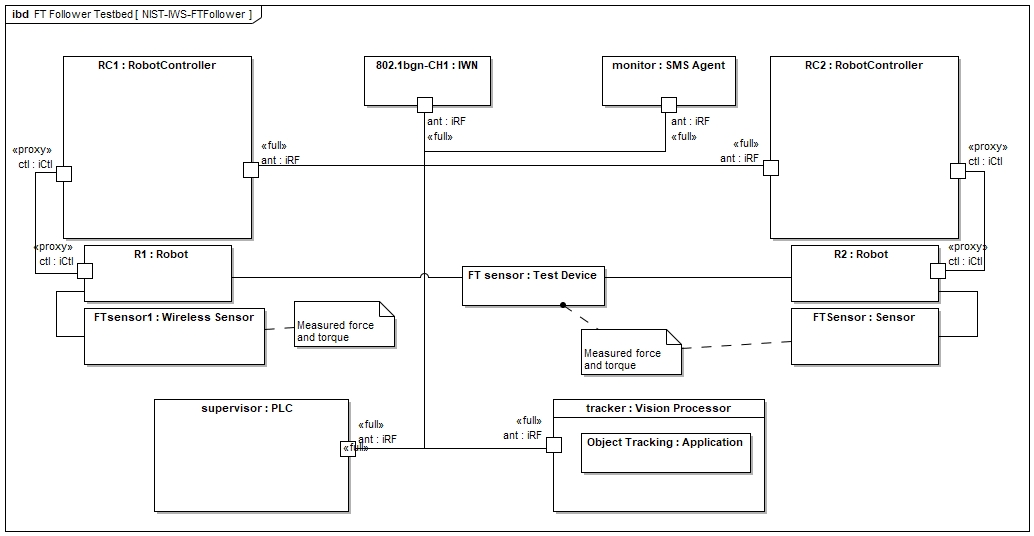
\includegraphics[width=0.85\textwidth]{chapter-conclusions/images/NIST-IWS-FTFollower}
	\caption{Internal block diagram of a workcell equipped with an robotic leader-follower lift application.}
	\label{fig:concl:lfscenario-full}
\end{figure}

\begin{figure}[!th]
	\centering
	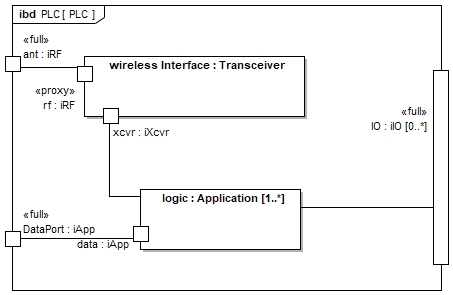
\includegraphics[width=0.85\textwidth]{chapter-conclusions/images/PLC}
	\caption{Internal block diagram of a \gls{plc}.}
	\label{fig:concl:plc-ibd}
\end{figure}

\begin{figure}[!th]
	\centering
	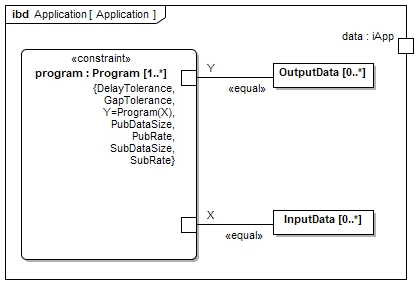
\includegraphics[width=0.85\textwidth]{chapter-conclusions/images/Application}
	\caption{Internal block diagram of an Application showing the parametrics constraints of its one or more programs.}
	\label{fig:concl:Application-ibd}
\end{figure}

\begin{figure}[!th]
	\centering
	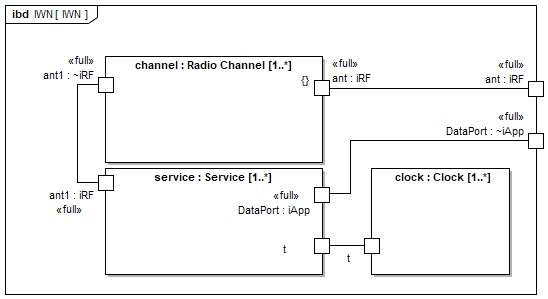
\includegraphics[width=0.85\textwidth]{chapter-conclusions/images/IWN}
	\caption{Internal block diagram of an \gls{iwn} showing the parametric constraints of its one or more programs.}
	\label{fig:concl:iwn-ibd}
\end{figure}

\begin{figure}[!th]
	\centering
	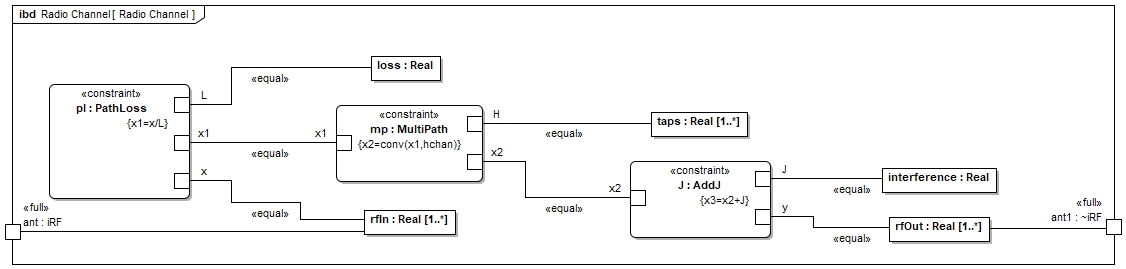
\includegraphics[width=0.85\textwidth]{chapter-conclusions/images/RadioChannel}
	\caption{Internal block diagram of an Radio Channel showing the parametric constraints of the radio medium.}
	\label{fig:concl:RadioChannel-ibd}
\end{figure}

\begin{figure}[!th]
	\centering
	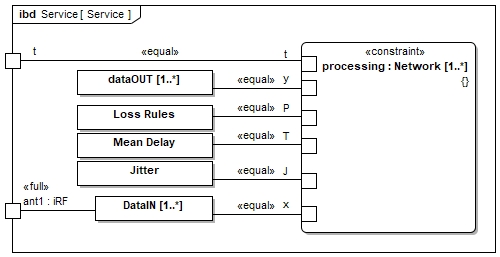
\includegraphics[width=0.85\textwidth]{chapter-conclusions/images/Service}
	\caption{Internal block diagram of an \gls{iwn} Service showing the parametric constraints of the behavior of a network service as generic processing.}
	\label{fig:concl:Service-ibd}
\end{figure}

And as shown in Fig.~\ref{fig:concl:conceptual}, each controller block such as a Robot Controller or a \gls{plc}~(Fig.~\ref{fig:concl:plc-ibd}) inherits its structure and behavior from the Controller block.  As such, the \gls{plc} and the Robot Controller have an Application and an interface to the wireless network.  Each application is linked to the wireless network through a Transceiver block (refer to \ref{fig:concl:plc-ibd}) which intuitively governs its own receiver performance as impacted by the radio channel.  The radio channel is an element of the \gls{iwn} block shown in Fig.~\ref{fig:concl:iwn-ibd} which is connected directly to a set of \gls{iwn} services as shown in Fig.~\ref{fig:concl:Service-ibd}. The service block of the \gls{iwn} is modeled as a generic sets of constraints that could be implemented as code or mathematical limitations.  

One can see that the complete path of information flow within the model proposed traverses the radio medium, the \gls{iwn}, the embedded transceivers, and each control application. Therefore, it is possible using this proposed model to represent the radio channel, model its performance impacts on the wireless network, and subsequently the impacts of the performance of the wireless network on the performance of the control applications themselves.  Such an interdisciplinary modeling effort is not an easy prospect and could be quite challenging; however, with the modeling framework presented as a part of this work, it becomes easier.  This represents an opportunity for refinement of the proposed model to be more intuitive and perhaps easier to use.  The contribution is made publicly available through Internet download through the URL provided in~\cite{Candell2018SysML.DATA}.

\begin{figure}[!th]
	\centering
	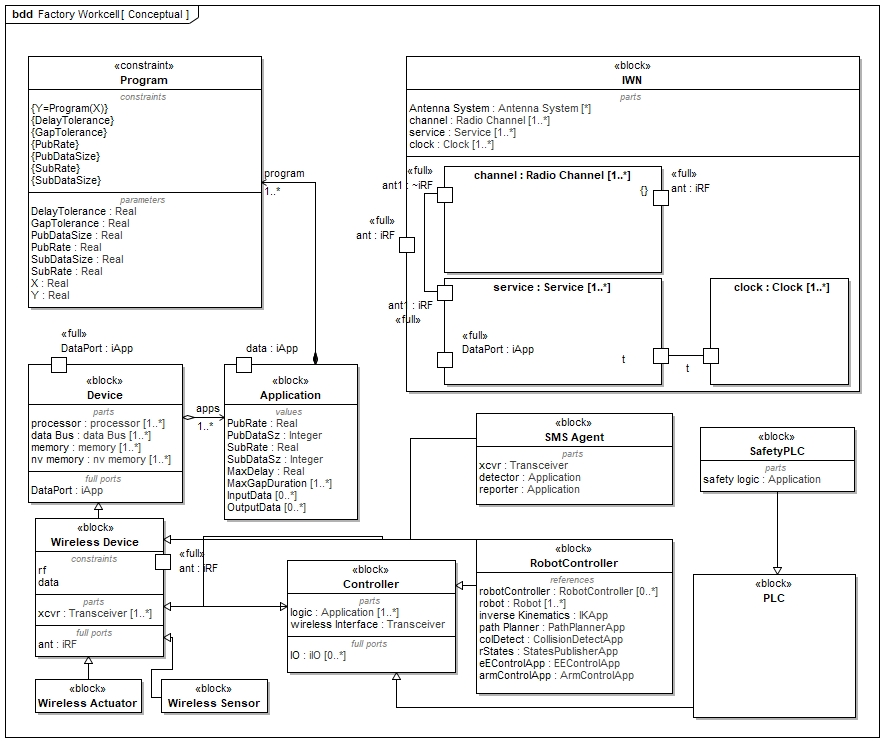
\includegraphics[width=0.95\textwidth]{chapter-conclusions/images/Conceptual}
	\caption{BBD of the conceptual relationships of model primitives}
	\label{fig:concl:conceptual}
\end{figure}

Our model was developed using \gls{sysml}. The developed model is constructed of the elements necessary to construct useful representations of factory workcells in which wireless networks are used to transport information necessary for automated control system operation.  Reusable, derivable elements are developed and then extended to represent the constructs of the workcell such as robot control, supervisory control, vision, safety, and spectrum monitoring.  An \gls{iwn} is then developed and constraints of the radio channel and network services are formalized. Using the architectural model, information flows are explored and incorporated within. 

It is important to mention that our model includes an often overlooked component of any industrial wireless deployment which is the spectrum monitoring system.  Our model also considers the human-robot and robot-robot interactions in industrial environments. The current model includes various systems constraints including motion constraints, radio channel constraints, and networking constraints. The parametric constraints are provided as examples and can be replaced with executable computer code thereby making the model useful for simulation depending on the modeling tool selected. Furthermore, the applications within the robotic work-cell define many information flows requiring careful analysis to achieve reliability and latency necessary for the safety and control of the manufacturing process.

With increased dependency on wireless communications for more complex manufacturing systems, the projection of manufacturing requirements onto the wireless communication system becomes less obvious.  Understanding the connection between the communication system and the operational system is not always obvious. Such analysis of this projection is essential for future research of manufacturing systems. As such, the architectural elements and information flows exposed by an abstract model are a necessary first step. The model in its current state of development is comprehensive enough to support architectural and ontological analyses of the factory workcell.  As such, information about the relationships between components of a workcell and attributes related to the wireless network may be discovered. Therefore, the model serves as a foundation for future systems engineering analyses. Moreover, the model may be used as a tool for academic and industry exploration of wireless testbed development.

\section{Graph Database Application}

Graph databases are designed to provide a powerful modeling framework for the storage and visualization of data in which relationships and connections between data could be significant but difficult to detect or visualize in the real world.  When one hears the word "database," typically one envisions a relational database such as MySQL or Oracle in which the database stores information in a highly structured manner in which tables are constructed in a predetermined way with columns, rows, and rigidly defined data types.  In contrast, \gls{gdb} are not rigid in their structure and organization.  Data is graph databases are intrinsically stored within nodes and vertices (connections).  Each node and vertex can have associated properties and thus store data as shown in Fig.~\ref{fig:concl:graphdb-sperical} which illustrates the common notion of a graph database.  In the graph units of information (nodes) exist with relationships lines between those units of information depicted as lines.  The connecting lines represent relationships which are the essential building block used within the contribution presented in the thesis~\cite{CandellISIT2020.Conf}.  

\begin{figure}[!ht]
	\centering
	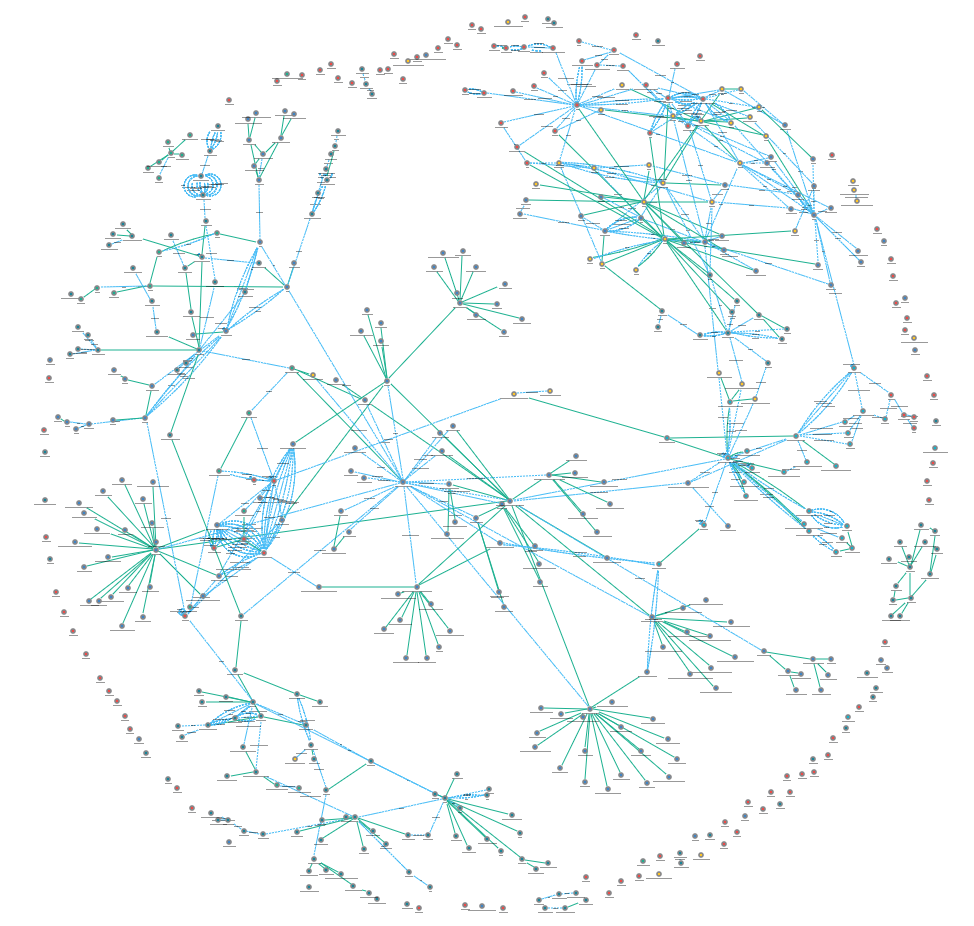
\includegraphics[width=0.8\textwidth]{chapter-conclusions/images/spherical-graph.png}
	\caption{A notional spherical graph depicting nodes and vertices.}
	\label{fig:concl:graphdb-sperical}
\end{figure}

The \gls{gdb} was employed within the work of this thesis.  It was demonstrated as an effective tool to model and capture performance information for research and possibly for situational awareness of factory operation.  The objective of using a graph database was essentially to 1) leverage the inherent connectivity of the data resulting from the experiments being performed within the \gls{nist} Industrial Wireless Laboratory, and 2) demonstrate that wireless networks could be used for a significant class of use case without impacting physical system performance. To support the research performed for this contribution, a testbed was constructed. This testbed was described in Chapter~\ref{chapter:graphdb} and is illustrated in the photo provided in Fig.~\ref{gdbappl:fig::workcell}.  The design of the testbed is captured in Fig.~\ref{fig:concl:experiment-design}.  Two robot arms were used to move and inspect parts through a series of four (4) \gls{cnc} machines.  Each robot is equipped with a 6-\gls{dof} force torque sensor in its wrist.  Joint control of each robots is conducted through a separate robot controller computer assembly.  A \gls{plc} was used to supervise activity within the workcell and was called the Supervisor.  The network and physical performance of the simulated workcell was captured completely agnostic of the type of communication network being used.  Through the use of adapter and network \gls{tap} devices shown in the diagram, it was possible to capture packet flight data in a way such that the type of technology used for communication did not alter routing of information.  By doing this, the schema of the graph database was left relatively unchanged across experiments while different wired and wireless protocols were investigated. Many instances of graph databases were produced for each experiment conducted using the testbed.

\begin{figure}[!ht]
	\centering
	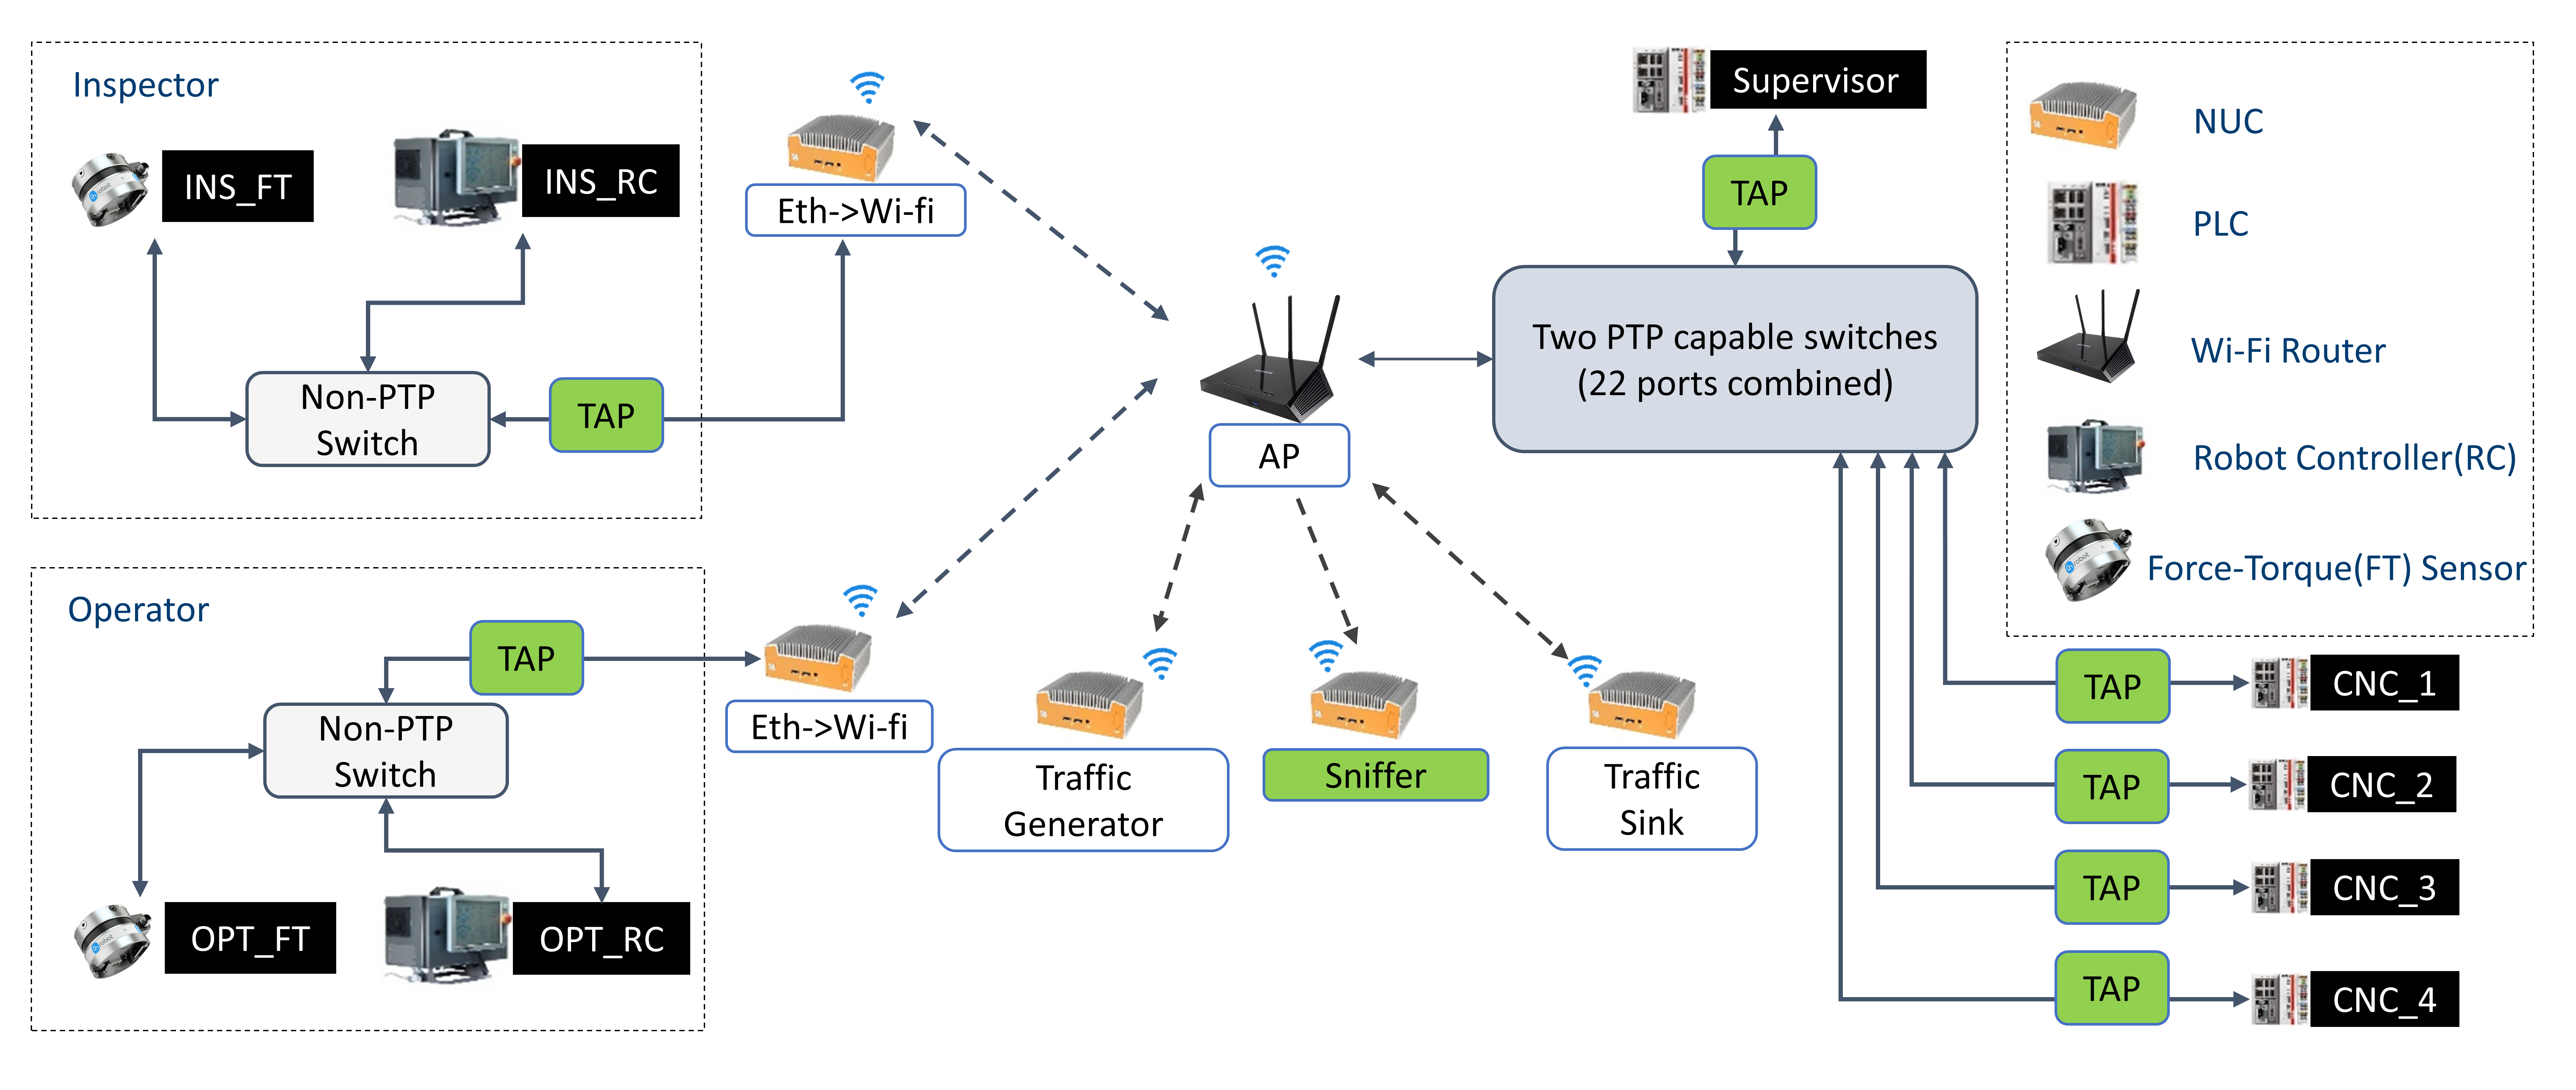
\includegraphics[width=0.95\textwidth]{chapter-gdb-appl/figures/Fig1TiiSpecialDiagram-testbed2.png}
	\caption{Experiment design used for capture of performance data.}
	\label{fig:concl:experiment-design}
\end{figure}

This shows what is important: the connection between physical actions and the transactions that support them.  Transactions are grouping of information transmissions (i.e., packets) that traverse the wireless network.  Factors that impact reliability of transactions such as message (i.e. packet) loss or message delay indirectly impact start and stop times of physical actions.  These relationships are directly captured within a graph and thus the applicability of a \gls{gdb} to the investigation of \gls{cps} performance becomes evident.  Ultimately, one could argue that the primary contribution of this component of the thesis is to demonstrate the interconnection between the industrial (wireless) network and physical operations through the modeling and capture of the performance data, the data relationships, and the analysis of physical action performance when network performance is degraded.  The use of the graph database makes that possible.  As an example, the schema shown in Fig.~\ref{fig:concl:data-physical-actions-following} was produced by querying the schema of a single database with hundreds of physical actions and hundreds of thousands of supporting transactions.  By querying the data represented by this structure, it was demonstrated that the wireless network employed did not prohibitively impact operation.  It was also demonstrated that through querying of the performance outliers that network events such as loss in signal strength or an increase in interference could be linked to a delay in the actuation of a robot action.  This type of event discovery and correlation to the physical world is particularly advantageous to facilitating the adoption of wireless in smart manufacturing.

\begin{figure}[!ht]
	\centering
	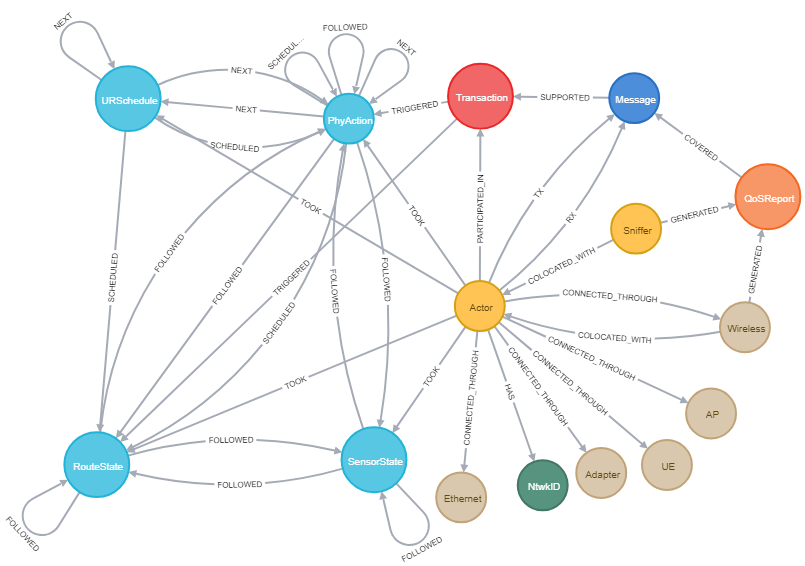
\includegraphics[width=0.85\textwidth]{chapter-gdb-appl/figures/database/graph_schema_updated_2.png}
	\caption{Experiment design used for capture of performance data.}
	\label{fig:concl:data-physical-actions-following}
\end{figure}

It is my opinion that the relationships between the physical actions through the FOLLOWED and NEXT relationships as shown in Fig.~\ref{fig:concl:data-physical-actions-following} and the TRIGGER relationships between physical actions and Transactions present a significant component of discovery within the results of this contribution. It is through the TRIGGER and FOLLOWED relationships that one can ascertain the impacts of network performance on physical systems performance. These are difficult to model with relationship databases.  It is possible to so so, but it is not inherent in the nature of the database itself to store such relationships.  When a triggering Transaction is correlated to a physical action using these relationships, it is then possible to follow the nodes backward in the graph to associated Message nodes and the \gls{qos} reports associated with those messages. These \gls{qos} reports provide evidence of degradation within the communication network during operation.  It is important to note that the \gls{qos} reports used for this investigation were produced externally using wireless sniffer devices that were co-located with transceiver equipment.  This was done due to the implementation difficulty in extracting \gls{qos} header information for each wireless packet received at each actor.  Since the experiments were performed, a method to extract wireless \gls{qos} header data at each transceiver was discovered.  Capture of wireless header information would enrich the data with more accurate \gls{qos} reports applicable directly to informational messages and thus allow for the construction of a more accurate data graph.

\section{Machine Learning Applications}

Machine learning (ML) is a large field of science and engineering that deals with the application of computing algorithms to perform actions without being explicitly programmed to do so.  In general applications, ML is used from applications ranging from voice recognition in personal electronics, spam filtering in email, and performing traffic prediction for commuters to providing services such friend identification and face recognition in social media.  In industrial applications, machine learning has the promise of a wide range of applications such as robot autonomy and detection of security anomalies. In this thesis, a machine learning framework was demonstrated for the prediction of the \gls{sir} within a communications link used for the control of a robot arm depressing a spring apparatus.  The ML framework as shown to be useful and accurate in the prediction of link quality.  \Gls{lqe} is an important metric in wireless communication system.  It is a general term used to describe the level of quality of a communication link.  The SIR metric is a ratio between the intended signal being transmitted and the level of interference competing with the intended signal.  Interference, whether caused by malicious jamming or not, is an impeding factor in the adoption of wireless in smart manufacturing systems.  Therefore, having a clear situational awareness picture of the level of interference and the quality of communication links being used is of clear interest.  The contribution presented within this thesis addresses a clear need in improving the detection and estimation of signal quality events in the workcell.  Future work to extend the framework could involve the following:

\begin{description}
	
	\item[More Dimensions] Application of this ML framework to a system with more degrees of freedom such as the entire workcell.  In the current contribution, the ML framework was applied to a single wireless communication link used to control one robot arm.  When expanded the framework to systems with more dimensions, the application of neural networks with deep learning may be beneficial.
	
	\item[Spectrum Monitoring System] Application of online learning techniques such that the ML framework can learn and adapt as the workcell operates would be beneficial as well.  In the current contribution, the ML framework learns offline from training data and then applies its knowledge to an active system.  This prohibits the system from learning as the wireless network changes over time.  Online techniques could allow for the ML framework to account for a changing spectral environment.
	
	\item[Control System Integration] Integration of this framework with the workcell control system such that the control system can adapt dynamically to interference for example to allow the control system to task preventative actions for safety or to operate in a reduced performance mode.
	
\end{description}

\section{Closing Remarks}

This thesis began with the very broad objective of investigating the area of performance estimation, testing, and control of \glspl{cps} employing non-ideal communications networks.  An ideal communication network is one in which all data arrives reliably and on-time.  In industrial settings, an ideal network is usually a wired networks built upon fieldbus protocols such as EtherCAT and CANbus or switched protocols founded upon Ethernet.  Ethernet and fieldbus are not 100\% reliable but their performance is nearly ideal for their intended applications.  Co-design, therefore, of the control system with the industrial network is often an unnecessary consideration in a wired network.  Enter industrial communication networks built upon wireless technology, and the situation appears very different.  While wireless technology provides key benefits in mobility and cost reduction, reliability of the network as compared to wired counterparts drops dramatically.  While wired network solutions can more easily transport data with more reliability and determinism, wireless solutions are built upon a shared limited physical medium, the electromagnetic spectrum, that is finite in bandwidth and is easily inhibited by distance, interference, and the structure of the surround environment.  Much hype exists surrounding the benefits of use of wireless in factories for collecting information about the operation and more recently for control of the factory itself.  Therefore, it becomes important to understand the operational requirements of the factory and then develop methods for assessing the performance of the factory network employing non-ideal communication such as that \gls{iwn}.  This thesis has contributed to this undertaking by doing the following:

\begin{enumerate}
	\item In Part~\ref{part:context}, an historical account of the past four industrial revolutions is provided.  In addition, the thesis introduces the reader to the importance of wireless networking in smart manufacturing and the main challenges that it faces toward widespread adoption. A review of the state-of-the-art of the requirements of industrial requirements, systems modeling, application of \glspl{gdb} to the problem of \glspl{cps}, and machine learning are also presented.  Within this look at the state of the art, our contribution within this thesis to wireless user requirements is also presented.
	
	\item In Part~\ref{part:techical}, provides the technical contributions of this thesis. Contributions in the areas of requirements, systems modeling, \gls{gdb} application, and machine learning are presented.  Each of the four chapters within Part~\ref{part:techical} describe our novel contributions as follows:
	\begin{enumerate}
		
		\item Chapter~\ref{chapter:reswk} explored the vast and continually changing landscape of wireless technology and provided new perspective of the applicability of existing and emerging technologies to classes of industrial sensing and control applications.
		
		\item Chapter~\ref{chapter:sysml}, presented a new framework for the modeling of \glspl{cps} employing wireless communication as the primary mode of data transfer using \gls{sysml}.
		
		\item Chapter~\ref{chapter:graphdb} presented the work of applying the \gls{gdb} to the problem of storing and querying performance data of the \gls{cps}.  Cyberphysical system performance data is highly connected, and thus the graph database was demonstrated to be a viable means of storing the data and discovering correlations within the data between network performance and operational performance.
		
		\item Finally, Chapter~\ref{chapter:ftml} presented the work of applying machine learning to prediction of \gls{qos} of wireless communication links within a representative industrial use case, a force seeking apparatus.
	\end{enumerate}
\end{enumerate}




%\chapter{Conclusions}
%
%\section{Future Work}
%Application of Machine Learning within the workcell control program
%
%how to extended the graph database and other data management approaches to the the factory and factory workcell rather than just for performance appraisal in the lab.
%
%Improvements to the schema, queries, and other database improvements to overcome the challenges encountered during research.  For example, rapidly expanding cartesian products within queries.  I note that the selected database has inherent problems with large scale queries wherein a query is constructed to for efficiency yet the database ignores the rules of the query and forms a cartesian product regardless.
%
%\section{Conclusions}

%\include{chapter-conclusions/chapter-conclusions}


%\chapter{Conclusions}
%paper on testbed construction; ground truth; data sources network and physical; data outputs; 
%paper on graph database approach for organization of data
%Discussion, Perspectives, restate findings
